\documentclass[11pt]{article}
\usepackage[a4paper,margin=1in]{geometry}
\usepackage[T1]{fontenc}
\usepackage{mathptmx}
\usepackage{microtype}
\usepackage{amsmath,amssymb}
\usepackage{graphicx}
\usepackage{booktabs}
\usepackage{caption}
\usepackage{enumitem}
\usepackage[numbers]{natbib}
\usepackage{xcolor}
\usepackage[colorlinks=true,linkcolor=blue!50!black,citecolor=blue!50!black,urlcolor=blue!50!black]{hyperref}
\captionsetup{font=small,labelfont=bf}
\setlist{itemsep=2pt,topsep=3pt}
\setlength{\parskip}{3pt}
\setlength{\emergencystretch}{2em}
\usepackage{fancyhdr}
\pagestyle{fancy}
\fancyhf{}
\fancyhead[L]{\small\itshape The False Strategy Problem in Machine Learning for Finance}
\fancyhead[R]{\small\itshape Navid Abdollahzadeh}
\fancyfoot[C]{\thepage}
\renewcommand{\headrulewidth}{0.4pt}
\setlength{\headheight}{14pt}

\title{\textbf{The False Strategy Problem in Machine Learning for Finance:}\\[2pt]
\large Why It Is Dangerously Easy to Discover ``Profitable'' Rules That Do Not Exist}
\author{Navid Abdollahzadeh}
\date{October 2026}

\begin{document}
\begin{titlepage}
\thispagestyle{empty}
\vspace*{0.6cm}
\begin{center}
{\LARGE\bfseries The False Strategy Problem in Machine Learning for Finance:\par}
\vspace{6pt}
{\Large Why It Is Dangerously Easy to Discover ``Profitable'' Rules That Do Not Exist\par}
\vspace{18pt}
\rule{0.55\textwidth}{0.4pt}\par
\vspace{14pt}
{\large Navid Abdollahzadeh\par}
\vspace{4pt}
{\normalsize Working paper \textperiodcentered{} October 2026\par}
\vspace{14pt}
\rule{0.55\textwidth}{0.4pt}\par
\end{center}
\vspace{1.2cm}
\begin{center}
\begin{minipage}{0.86\textwidth}
\begin{center}{\bfseries Abstract}\end{center}
\vspace{2pt}
\small
When many trading strategies are tested on the same historical data and only the best is reported, its backtested performance is a biased estimate of its true performance. This paper studies that \emph{false strategy problem} in the setting where it is now most severe: machine-learning (ML) pipelines that evaluate many model, feature and hyperparameter configurations automatically. Building on the False Strategy Theorem and related tools, I report seven controlled experiments with known ground truth and one real-data case study. Among strategies with zero true skill, the best of 1{,}000 five-year backtests has a mean annualized Sharpe ratio of 1.45, as the theorem predicts. A random search over 200 configurations of gradient-boosted trees, random forests, neural networks and logistic regression on unpredictable data raises the selected model's validation Sharpe ratio from 0 to 2.3, while its Sharpe ratio on an untouched test year stays near zero. Shuffled cross-validation reports 65.7\% accuracy on a random walk; purged cross-validation gives chance. These results are unchanged under GARCH volatility, regime switching and transaction costs. The main methodological finding concerns the correction itself. The Deflated Sharpe Ratio needs the effective number of independent trials, and the common practice of counting clusters of similar strategies can understate it by a factor of 17, raising the test's false-positive rate from under 1\% to 23\%. An eigenvalue estimator borrowed from statistical genetics tracks the true value, keeps false positives below 1\% and matches the power achievable with the true value to within 2.4 percentage points on average. On the S\&P~500 from 1990 to 2026, the best of 156 timing rules beat buy-and-hold in sample but trailed it out of sample, and its deflated significance ranged from 0.61 to 0.998 depending on how the number of trials was counted. I close with a tiered validation protocol.

\vspace{12pt}
\noindent\textbf{Keywords:} backtest overfitting; multiple testing; selection bias; Sharpe ratio; Deflated Sharpe Ratio; effective number of tests; hyperparameter search; cross-validation leakage; machine learning in finance.

\vspace{6pt}
\noindent\textbf{JEL classification:} C12, C15, C52, C58, G11, G17.
\end{minipage}
\end{center}
\vfill
\begin{center}
\footnotesize Code and results for every number, table and figure are provided as supplementary material.
\end{center}
\end{titlepage}

%=====================================================
\section{Introduction}

A researcher who tests enough trading rules on historical data will almost certainly find one that looks profitable, even when every rule is worthless. This is the \emph{false strategy problem}. The best backtest in a large search is selected \emph{because} it was lucky, so its in-sample performance is an inflated estimate of its true performance, which may be zero or negative.

The problem is old. \citet{lo1990} warned of data-snooping biases in tests of asset-pricing models, and \citet{sullivan1999} showed that much of the apparent skill of technical trading rules disappears once the size of the search is taken into account. What is new is scale. Modern ML pipelines can evaluate thousands of feature sets, architectures, hyperparameters and trading thresholds in an afternoon. Each evaluation is a hidden trial. A practitioner who reports only the winner, with an ordinary Sharpe ratio and an ordinary $t$-statistic, is in effect reporting the maximum of thousands of noisy draws as if it were a single draw.

Finance is an unusually hostile setting for this. Signal-to-noise ratios in asset returns are very low; the data are non-stationary; history cannot be re-run; and samples are short relative to the number of configurations a computer can try. \citet{harvey2016} argue that, given the number of factors the profession has tested, most claimed findings in empirical finance are likely false. \citet{bailey2014pseudo} go further and describe uncorrected backtest optimization as ``pseudo-mathematics''.

This paper asks two questions: \textbf{how large is the gap between apparent and true performance when ML-style search is applied to financial data, and how reliably can the standard corrections close it?} The theoretical tools it uses, from the False Strategy Theorem to purged cross-validation, are established \citep{bailey2014dsr,bailey2017pbo,lopezdeprado2018,lopezdeprado2021fst}. Its contributions are the following:
\begin{enumerate}
  \item \textbf{A unified, reproducible demonstration.} Controlled experiments with known ground truth quantify each mechanism in turn: selection among independent strategies, search over a correlated rule grid, naive versus deflated significance, and cross-validation leakage (Section~\ref{sec:sim}).
  \item \textbf{Direct evidence for ML search.} A random search over four model families, their hyperparameters, feature subsets and random seeds shows how quickly validation performance inflates when nothing is predictable (Section~\ref{sec:ext}).
  \item \textbf{A robustness check.} The results hold under GARCH volatility, regime switching, heavy tails and transaction costs, so they are not an artefact of Gaussian assumptions.
  \item \textbf{A methodological finding on the effective number of trials.} I show that counting clusters of similar strategies, a common way to set $K$ in the Deflated Sharpe Ratio, can badly understate the number of chances luck has had, and that an eigenvalue estimator from statistical genetics \citep{liji2005} performs much better. To my knowledge this comparison has not been reported for the DSR.
  \item \textbf{A real-data case study} on the S\&P~500 index from 1990 to 2026 (Section~\ref{sec:real}).
  \item \textbf{A tiered validation protocol} that separates the steps every project needs from additional statistical safeguards (Section~\ref{sec:protocol}).
\end{enumerate}

Section~\ref{sec:lit} reviews related work. Section~\ref{sec:theory} sets out the theory. Section~\ref{sec:sim} presents the core simulation study and Section~\ref{sec:ext} its extensions. Section~\ref{sec:real} applies the tools to real data. Section~\ref{sec:ml} discusses failure modes specific to ML, Section~\ref{sec:protocol} proposes defences, and Section~\ref{sec:disc} discusses limitations and concludes.

%=====================================================
\section{Background and related literature}\label{sec:lit}

\paragraph{Data snooping and multiple testing.}
Statistics has long recognised that testing many hypotheses inflates the chance of false positives. Classical corrections control the family-wise error rate \citep{holm1979} or the false discovery rate \citep{benjamini1995}. In econometrics, \citet{white2000} introduced the \emph{Reality Check}, a bootstrap test of whether the best of many forecasting models truly beats a benchmark once the whole search is accounted for. \citet{hansen2005} refined it into the test for Superior Predictive Ability, and \citet{romano2005} developed a stepwise procedure that identifies \emph{which} models outperform. \citet{sullivan1999} applied the Reality Check to almost 8{,}000 technical trading rules and found that the best rule's apparent outperformance on the Dow Jones Industrial Average did not survive in later data.

\paragraph{The factor zoo and the replication debate.}
\citet{harvey2016} catalogue hundreds of published return predictors and argue that a new factor should clear a $t$-statistic of about 3.0, rather than the conventional 2.0, to account for the profession's cumulative search. \citet{mclean2016} find that the returns of 97 published anomalies are 26\% lower out of sample and 58\% lower after publication, consistent with a mix of statistical bias and arbitrage. \citet{hou2020} report that most of 452 anomalies fail to replicate once microcap stocks are handled appropriately. The picture is contested: \citet{jensen2023} use a Bayesian framework and conclude that most factors \emph{do} replicate once evidence is pooled across related factors and markets. The debate is itself informative. Whether a finding is ``real'' depends heavily on how one accounts for the number of tries that produced it.

\paragraph{Backtest overfitting.}
A parallel literature, developed largely by Bailey, Borwein, L\'opez de Prado and co-authors, focuses on investment strategies rather than academic factors. \citet{bailey2014pseudo} show that with five years of daily data, trying more than about 45 independent strategy variations is enough to expect an in-sample Sharpe ratio of 1.0 from a strategy with no skill. \citet{bailey2014dsr} introduce the Deflated Sharpe Ratio (DSR), which corrects a Sharpe ratio for the number of trials and for non-normal returns. \citet{bailey2017pbo} propose combinatorially symmetric cross-validation (CSCV) and the Probability of Backtest Overfitting (PBO). \citet{lopezdeprado2018} extends these ideas to ML workflows, introducing purged and embargoed cross-validation for financial labels. \citet{lopezdeprado2019lewis} and \citet{lopezdeprado2021fst} formalise the result now known as the False Strategy Theorem.

\paragraph{The effective number of tests.}
When tests are correlated, the raw count overstates the multiple-testing burden. Statistical genetics faces this problem with correlated genetic markers and estimates an effective number of independent tests from the eigenvalues of their correlation matrix \citep{liji2005}. In finance, \citet{lopezdeprado2019lewis} instead cluster the trials' return series. Which approach better serves the DSR has not, to my knowledge, been tested; Experiment~7 does so.

\paragraph{Machine learning in asset pricing.}
ML can add real value. \citet{gu2020} find that tree ensembles and neural networks improve out-of-sample prediction of US stock returns relative to linear models, and \citet{kelly2024} argue that, under some conditions, highly parameterised models can outperform simpler ones. These results do not contradict the false strategy problem. They were obtained with careful out-of-sample designs, and they show why the design matters: the same flexibility that allows ML to capture real structure also allows it to fit noise. The machine-learning literature knows the same problem under a different name. \citet{cawley2010} show that selecting hyperparameters on a validation set biases the validation score upward, so that a model's performance must be estimated on data untouched by the selection. Random search \citep{bergstra2012}, now a standard tuning method, makes it cheap to try hundreds of configurations, each of which is a trial in the sense used here. \citet{arnott2019} propose a backtesting protocol for this setting, and this paper's recommendations in Section~\ref{sec:protocol} build on it.

%=====================================================
\section{Theoretical framework}\label{sec:theory}

\subsection{Selection under noise}
Let a researcher evaluate $K$ strategies on the same sample of $T$ return observations and let $\widehat{SR}_k$ denote the estimated Sharpe ratio of strategy $k$. Suppose none has skill: the true Sharpe ratio is $SR_k = 0$ for every $k$. Under independent, identically distributed normal returns, the estimator is approximately normal with variance $\mathrm{V}[\widehat{SR}_k] \approx (1 + SR_k^2/2)/T$ \citep{lo2002}, which is $1/T$ per period when $SR_k = 0$. On an annualized basis with $T$ daily observations and 252 trading days per year, its standard deviation is $\sqrt{252/T} = 1/\sqrt{Y}$, where $Y$ is the length of the backtest in years. A five-year backtest of a worthless strategy therefore produces an annualized Sharpe ratio with a standard deviation of about 0.45. The question is what happens to the \emph{maximum} of $K$ such draws.

\subsection{The False Strategy Theorem}
Applying extreme-value theory for the maximum of normal variables, \citet{bailey2014dsr} and \citet{lopezdeprado2021fst} show that
\begin{equation}\label{eq:fst}
\mathrm{E}\!\left[\max_k \widehat{SR}_k\right] \approx \sqrt{\mathrm{V}\!\left[\{\widehat{SR}_k\}\right]}\;\Big( (1-\gamma)\,\Phi^{-1}\!\left[1 - \tfrac{1}{K}\right] + \gamma\,\Phi^{-1}\!\left[1 - \tfrac{1}{K e}\right] \Big),
\end{equation}
where $\Phi^{-1}$ is the inverse standard normal CDF, $e$ is Euler's number and $\gamma \approx 0.5772$ is the Euler--Mascheroni constant. Two features matter.

First, the expected maximum grows without bound in $K$, roughly like $\sqrt{2\ln K}$. There is no number of trials at which the problem stops getting worse. Second, it scales with the dispersion of the estimates. Anything that increases that dispersion, such as shorter samples, fat tails or more flexible models, inflates the best result further. The theorem's name reflects its practical meaning: \emph{the best of many strategies will look skilful even when none is}.

\subsection{Minimum backtest length}
Setting the left-hand side of \eqref{eq:fst} equal to a target Sharpe ratio $\overline{SR}$ and solving for the sample length gives the \emph{Minimum Backtest Length} \citep{bailey2014pseudo}:
\begin{equation}\label{eq:minbtl}
\mathrm{MinBTL} \approx \left( \frac{(1-\gamma)\,\Phi^{-1}[1-1/K] + \gamma\,\Phi^{-1}[1-1/(Ke)]}{\overline{SR}} \right)^{2} \text{ years.}
\end{equation}
This is the backtest length below which the best of $K$ skill-less strategies is \emph{expected} to show an annualized Sharpe ratio of at least $\overline{SR}$. Figure~\ref{fig:minbtl} plots it. With $K=45$, five years of data are enough to produce an expected best Sharpe ratio of 1.0 from noise alone. With $K=1{,}000$, about 10.6 years are needed. With a more modest target of 0.5, typical of real long-horizon strategies, 1{,}000 trials require more than 42 years of data. Few financial datasets are that long, and fewer are stationary over that span.

\begin{figure}[t]
\centering
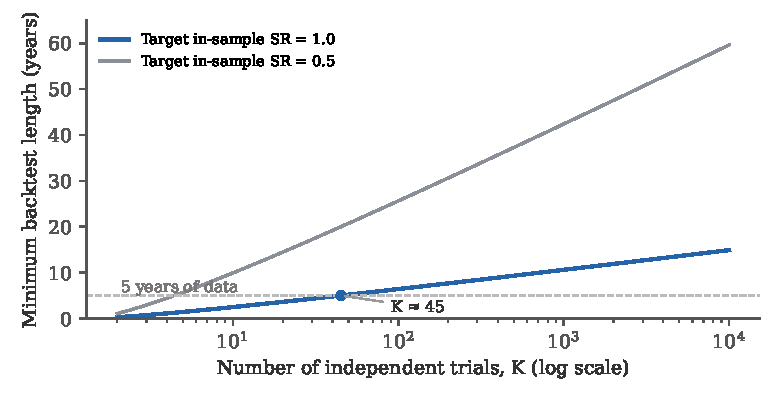
\includegraphics[width=0.82\linewidth]{fig2.pdf}
\caption{Minimum backtest length, Eq.~\eqref{eq:minbtl}. A backtest shorter than the curve is expected to produce the target Sharpe ratio from noise alone after $K$ independent trials. Five years of daily data support only about 45 independent trials for a target of 1.0.}
\label{fig:minbtl}
\end{figure}

\subsection{The Deflated Sharpe Ratio}
The Probabilistic Sharpe Ratio \citep{bailey2012} gives the probability that the true Sharpe ratio exceeds a benchmark $SR^{*}$, allowing for sample length, skewness $\hat\gamma_3$ and kurtosis $\hat\gamma_4$:
\begin{equation}\label{eq:psr}
\mathrm{PSR}(SR^{*}) = \Phi\!\left( \frac{(\widehat{SR} - SR^{*})\sqrt{T-1}}{\sqrt{1 - \hat\gamma_3\,\widehat{SR} + \frac{\hat\gamma_4 - 1}{4}\,\widehat{SR}^2}} \right).
\end{equation}
The Deflated Sharpe Ratio \citep{bailey2014dsr} sets the benchmark $SR^{*}$ equal to the expected maximum from Eq.~\eqref{eq:fst}. In words, it asks whether the selected strategy beats \emph{the best result that luck alone would have produced}, given how many strategies were tried. A DSR above 0.95 is the analogue of significance at the 5\% level after correcting for selection.

\subsection{Why machine learning amplifies the problem}
In the framework above, ML affects two quantities. It raises $K$, because every configuration of features, model class, hyperparameters, labelling rule and trading threshold is a trial, whether or not it is recorded. It also raises the dispersion term, because flexible models fit the idiosyncrasies of a particular sample more closely. A third effect is subtler: when the validation procedure itself leaks information (Section~\ref{sec:ml}), even a \emph{single} trial can produce an inflated estimate, and Eq.~\eqref{eq:fst} then understates the bias.

The trials are also correlated, since neighbouring hyperparameter settings give similar results. The relevant $K$ in Eq.~\eqref{eq:fst} is therefore the \emph{effective} number of independent trials, which is smaller than the raw count but rarely small. Three estimators are compared in Experiment~7. Let $\lambda_1,\dots,\lambda_N$ be the eigenvalues of the $N \times N$ correlation matrix of the trials' returns. The \emph{participation ratio} is $(\sum_i \lambda_i)^2 / \sum_i \lambda_i^2$, a standard measure of dimensionality. The \citet{liji2005} estimator is
\begin{equation}\label{eq:liji}
K_{\mathrm{LJ}} = \sum_{i=1}^{N} \Big( \mathbb{1}[\lambda_i \geq 1] + (\lambda_i - \lfloor \lambda_i \rfloor) \Big),
\end{equation}
which counts each dominant eigenvalue as one test and lets the remaining variance contribute fractionally. The third estimator is the number of clusters found by hierarchical clustering of the correlation matrix, in the spirit of \citet{lopezdeprado2019lewis}.

%=====================================================
\section{Simulation study}\label{sec:sim}

All experiments use synthetic data in which the true answer is known: there is no exploitable signal unless one is deliberately inserted. This makes it possible to measure the false strategy problem exactly, which is impossible with real market data. All code was written in Python (NumPy, SciPy, scikit-learn) with fixed random seeds. The code, result files and data needed to reproduce every number, table and figure in this paper are provided as supplementary material.

\subsection{Experiment 1: the best of $K$ worthless strategies}
\textbf{Design.} I draw $K$ independent strategies, each with $T = 1{,}260$ daily returns (five years) that are i.i.d.\ normal with mean zero and 1\% daily volatility. The true Sharpe ratio of every strategy is exactly zero. I select the strategy with the highest annualized in-sample Sharpe ratio and then evaluate it on a fresh five-year sample from the same process. I repeat this between 40 and 2{,}000 times for each $K \in \{1, 10, 100, 1{,}000, 10{,}000\}$.

\textbf{Results.} Table~\ref{tab:exp1} and Figure~\ref{fig:exp1} show the results. The selected strategy's in-sample Sharpe ratio rises steadily with $K$: from about zero for a single strategy, to 0.68 for 10, 1.12 for 100, 1.45 for 1{,}000 and 1.69 for 10{,}000. With 1{,}000 or more trials, \emph{every} replication produced a ``winner'' with a Sharpe ratio above 1.0, a level many practitioners would regard as attractive. Out of sample, the same strategies earn between $-0.02$ and $0.02$, consistent with zero. The False Strategy Theorem predicts the in-sample mean to within 0.04 at every $K$.

\begin{table}[h]
\centering
\caption{Experiment 1. Best-of-$K$ annualized Sharpe ratios for strategies with zero true skill (five-year in-sample and five-year out-of-sample periods).}
\label{tab:exp1}
\small
\begin{tabular}{rrcccc}
\toprule
$K$ & Reps. & Best in-sample SR & 5th--95th pct. & FST prediction & Out-of-sample SR \\
\midrule
1      & 2{,}000 & 0.01 & $-0.74$ to 0.75 & 0.00 & $-0.00$ \\
10     & 2{,}000 & 0.68 & 0.29 to 1.13 & 0.70 & $-0.00$ \\
100    & 1{,}000 & 1.12 & 0.84 to 1.47 & 1.13 & 0.02 \\
1{,}000  & 300  & 1.45 & 1.22 to 1.72 & 1.46 & $-0.01$ \\
10{,}000 & 40   & 1.69 & 1.53 to 1.84 & 1.73 & $-0.02$ \\
\bottomrule
\end{tabular}
\end{table}

\begin{figure}[t]
\centering
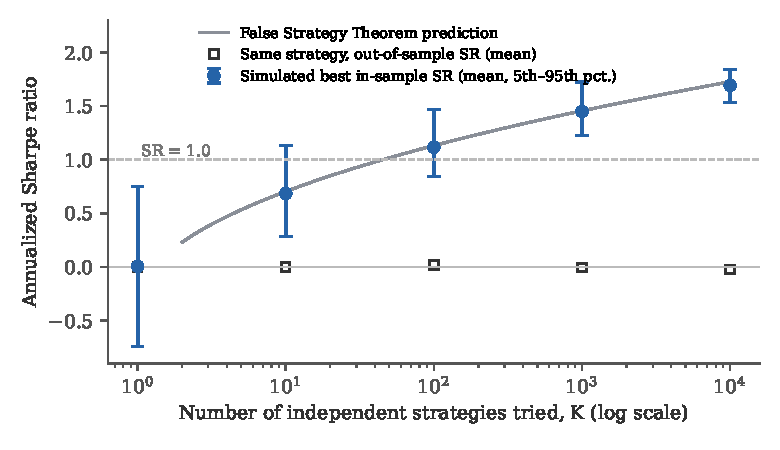
\includegraphics[width=0.85\linewidth]{fig1.pdf}
\caption{Experiment 1. The best in-sample Sharpe ratio among $K$ worthless strategies (blue) closely follows the False Strategy Theorem (grey line), while the same strategies earn nothing out of sample (open squares).}
\label{fig:exp1}
\end{figure}

\subsection{Experiment 2: searching a rule grid on random walks}
\textbf{Design.} Experiment 1 assumes independent strategies. Real searches explore correlated variants of one idea. I therefore simulate a price series as a Gaussian random walk, which by construction cannot be predicted, and apply 156 moving-average crossover rules (fast window 2--50 days, slow window 20--200 days). Each rule goes long when the fast average is above the slow one and short otherwise. I select the rule with the best Sharpe ratio over three years and evaluate it over the following two years, over 200 independent price paths. For 20 of the paths I also compute the Probability of Backtest Overfitting using CSCV with 16 blocks, i.e.\ $\binom{16}{8} = 12{,}870$ train/test splits \citep{bailey2017pbo}.

\textbf{Results.} The best rule's mean in-sample Sharpe ratio was 0.95, and it exceeded 1.0 on 42.5\% of paths. Its mean out-of-sample Sharpe ratio was 0.03, and it was positive on 51.5\% of paths, a coin flip. The rank correlation between in-sample and out-of-sample Sharpe ratios across the 156 rules was $-0.02$: in-sample ranking carried no information about future ranking. Mean PBO was 0.51 (range 0.15--0.89), the value expected when selection has no skill. Figure~\ref{fig:pbo} shows the CSCV distribution for one path.

Because the rules are highly correlated, 156 rules behave like far fewer independent trials. Inverting Eq.~\eqref{eq:fst} with the observed mean maximum of 0.95 over three years gives an effective $K$ of about 12. Even this modest effective search was enough to produce Sharpe ratios that would pass a casual review.

\begin{figure}[t]
\centering
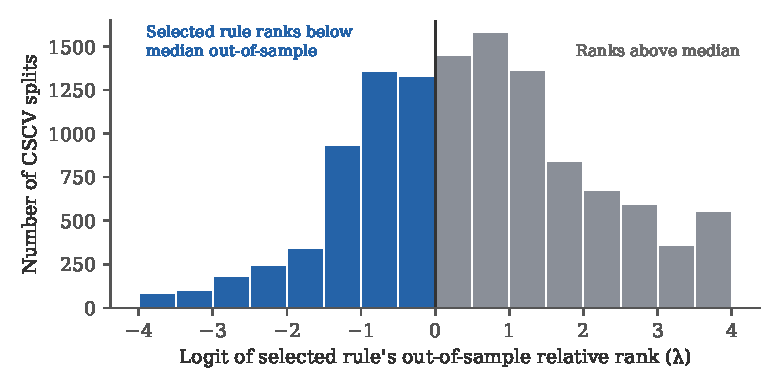
\includegraphics[width=0.82\linewidth]{fig3.pdf}
\caption{Experiment 2. Distribution of $\lambda$, the logit of the in-sample-best rule's relative out-of-sample rank, over CSCV splits for one random-walk path. Mass to the left of zero (blue) is the PBO. Splits with $|\lambda| > 4$ are not shown.}
\label{fig:pbo}
\end{figure}

\subsection{Experiment 3: does deflation separate skill from luck?}
\textbf{Design.} I repeat the best-of-$K$ selection with heavier-tailed returns (Student-$t$ with five degrees of freedom, rescaled to 1\% daily volatility) and five-year samples. In some designs, strategy 1 is given genuine skill (a true annualized Sharpe ratio of 1.0 or 2.0) while the rest have none. For the selected strategy I compute (a) a naive PSR against a benchmark of zero, which ignores selection, and (b) the DSR, with $SR^*$ from Eq.~\eqref{eq:fst} using the cross-sectional variance of the $K$ estimates. Each design is repeated 200 times.

\begin{table}[h]
\centering
\caption{Experiment 3. Share of replications in which the selected strategy is declared significant (statistic $> 0.95$).}
\label{tab:exp3}
\small
\begin{tabular}{rcccc}
\toprule
$K$ & True SR of strategy 1 & Selected = true strategy & Naive PSR significant & DSR significant \\
\midrule
1{,}000 & 0.0 (none skilled) & -- & 100\% & 0.0\% \\
1{,}000 & 1.0 & 17.5\% & 100\% & 0.0\% \\
1{,}000 & 2.0 & 85.5\% & 100\% & 31.5\% \\
100     & 1.0 & 33.5\% & 100\% & 0.0\% \\
\bottomrule
\end{tabular}
\end{table}

\textbf{Results.} Table~\ref{tab:exp3} contains the central lesson. The naive test declares the winner significant in 100\% of replications, \emph{including when no strategy has any skill}. The DSR declares none of the pure-noise winners significant. The table also shows the price of honesty. When one strategy has a true Sharpe ratio of 1.0 and 999 have none, search selects the skilled strategy only 17.5\% of the time, and the DSR never confirms it. Over five years, a real Sharpe ratio of 1.0 is statistically indistinguishable from the luck of the best of 1{,}000 noise strategies. Only a strong signal (a Sharpe ratio of 2.0) is usually selected, and even then it passes the DSR in about a third of cases. This is not a weakness of the DSR. It is an accurate statement of how little information a five-year backtest contains once a thousand alternatives have been examined.

\subsection{Experiment 4: leakage in cross-validation}
\textbf{Design.} A common ML workflow labels each day with the sign of the next 20-day return and estimates accuracy with $k$-fold cross-validation. Labels on adjacent days share 19 of their 20 future returns, so they are strongly dependent. I simulate a random walk of 2{,}500 days, construct five features (trailing returns over 5, 10, 20 and 60 days and trailing 20-day volatility), and train a random-forest classifier (150 trees) to predict the 20-day direction. True predictability is zero. Accuracy is estimated in three ways: (i) standard shuffled 5-fold cross-validation; (ii) purged and embargoed 5-fold cross-validation \citep{lopezdeprado2018}, which removes from training any observation whose label window overlaps the test fold, plus a 25-day buffer; and (iii) walk-forward testing with a gap. I repeat this over 10 independent paths.

\textbf{Results.} Shuffled cross-validation reports 65.7\% accuracy (range 63.2\%--67.8\%), far from the true 50\% (Figure~\ref{fig:leak}). The model is not predicting the future. Its training set contains neighbouring days whose labels are nearly identical to the test labels, and the trailing-return features let it locate those neighbours. Purging removes the effect (48.8\%), as does walk-forward testing (49.7\%). Unlike Experiments 1--3, this inflation arises from a \emph{single} model evaluation, with no search at all. Combined with search, leakage and selection bias compound.

\begin{figure}[t]
\centering
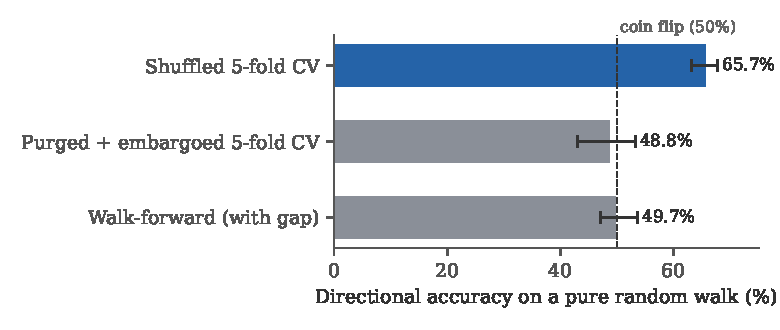
\includegraphics[width=0.85\linewidth]{fig4.pdf}
\caption{Experiment 4. Estimated directional accuracy of a random forest on an unpredictable random walk (mean and range over 10 paths). Shuffled cross-validation leaks label information through overlapping 20-day labels.}
\label{fig:leak}
\end{figure}

%=====================================================
\section{Extensions: ML search, realistic markets and the effective number of trials}\label{sec:ext}

Experiments 1--4 isolate the basic mechanisms under simple assumptions. This section asks three harder questions. Does the problem appear when the search is over real ML models rather than trading rules? Does it survive realistic market dynamics? And can the standard correction be applied reliably when, as in practice, the effective number of trials is unknown?

\subsection{Experiment 5: hyperparameter, feature and seed search}
\textbf{Design.} I simulate 24 independent Gaussian random walks and try to predict the next day's direction from 12 candidate features: the last five daily returns, momentum over 5, 10, 20 and 60 days, volatility over 5 and 20 days, and the distance from the 20-day moving average. Labels do not overlap, so the leakage of Experiment~4 is absent. The data are split in time: three years for training, one year for validation and one untouched year for testing. On each path I run a random search \citep{bergstra2012} over 200 configurations. Each draws a model family (gradient-boosted trees, random forest, logistic regression or a one-layer neural network), its hyperparameters, a random subset of 3 to 12 features and a random seed. Each model trades long or short according to its prediction. As a practitioner would, I select the configuration with the highest validation Sharpe ratio and then evaluate it on the test year. To trace the effect of search size, I also select from random subsets of $K$ configurations, for $K$ from 1 to 200.

\textbf{Results.} Figure~\ref{fig:mlsearch} shows the result. With a single configuration the validation Sharpe ratio is $-0.02$ on average, as it should be. With 20 configurations the selected model shows 1.55, with 100 it shows 2.12, and with all 200 it shows 2.31. Every one of the 24 searches produced a model with a validation Sharpe ratio above 1.0. On the untouched test year, the same models earned between $-0.05$ and $0.13$ on average, consistent with zero, and only 54\% were profitable. Validation accuracy rose to 55.8\% while test accuracy stayed at 50.6\%. A naive significance test certified 92\% of the selected models; the DSR with $K = 200$ certified none. No model family was immune: the winners were gradient-boosted trees on 11 paths, neural networks on 6, random forests on 5 and logistic regression on 2.

The configurations are correlated, because they share data and often features. Inverting Eq.~\eqref{eq:fst} shows that 200 configurations behaved like about 54 independent trials, and 20 like about 9. The theorem with the raw count therefore over-predicts the inflation (dashed line), while the observed inflation is still large enough to produce Sharpe ratios above 2 from pure noise.

\begin{figure}[t]
\centering
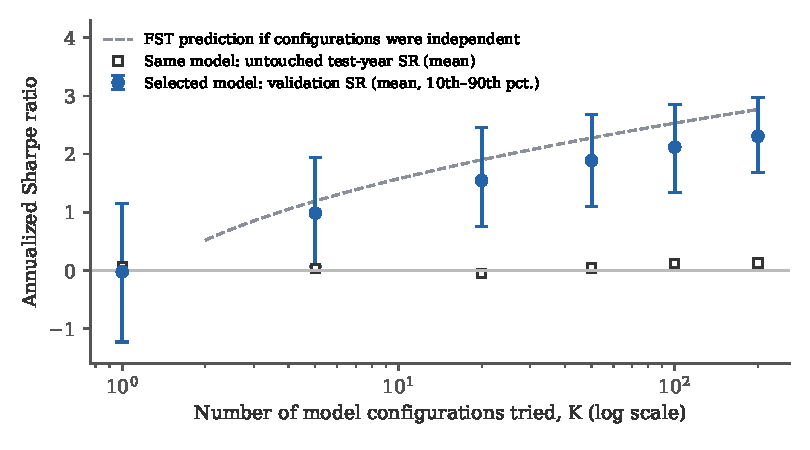
\includegraphics[width=0.85\linewidth]{fig5.pdf}
\caption{Experiment 5. Random search over ML configurations on unpredictable data. The selected model's validation Sharpe ratio (blue) grows with the number of configurations tried; its Sharpe ratio on an untouched test year (open squares) stays near zero. The dashed line is the False Strategy Theorem with the raw count, which over-predicts because configurations are correlated. 24 paths; for $K < 200$, 20 random subsets per path.}
\label{fig:mlsearch}
\end{figure}

\subsection{Experiment 6: realistic market dynamics and transaction costs}
\textbf{Design.} I rerun the rule search of Experiment~2 on price paths that keep a zero expected return but have realistic volatility. Returns follow a GARCH(1,1) process \citep{bollerslev1986} with $\alpha = 0.09$, $\beta = 0.90$ and Student-$t$ innovations with five degrees of freedom, multiplied by a two-state Markov volatility regime \citep{hamilton1989}: a calm state (0.8 times normal volatility) and a turbulent state (1.6 times), with daily persistence probabilities of 0.995 and 0.98. Paths are rescaled to 1\% average daily volatility. The simulated paths have a mean excess kurtosis of 13.0 and a lag-one autocorrelation of squared returns of 0.17; the corresponding figures for daily S\&P~500 returns from 1990 to 2026 are 10.9 and 0.31. Each rule pays 2 basis points per unit of turnover, so a switch from long to short costs 4 basis points. A fresh run of the Gaussian design of Experiment~2 serves as the baseline; both use 200 paths, with PBO computed on 20.

\begin{table}[h]
\centering
\caption{Experiment 6. Best of 156 crossover rules on zero-return price paths: Gaussian random walk versus GARCH with regime switching. Sharpe ratios are annualized; ``net'' deducts 2 bps per unit of turnover.}
\label{tab:exp6}
\small
\begin{tabular}{lcc}
\toprule
 & Gaussian random walk & GARCH + regimes \\
\midrule
Best rule, in-sample SR (gross / net) & 0.88 / 0.86 & 0.85 / 0.83 \\
Same rule, out-of-sample SR (gross / net) & $-0.03$ / $-0.05$ & 0.01 / $-0.02$ \\
Share of paths with in-sample SR $> 1$ & 39.5\% & 36.0\% \\
Share of paths with positive net out-of-sample SR & 47.5\% & 51.0\% \\
Rank correlation, in- vs out-of-sample & 0.00 & 0.00 \\
Probability of backtest overfitting & 0.49 & 0.49 \\
Effective number of trials (from Eq.~\ref{eq:fst}) & 9.0 & 8.1 \\
\bottomrule
\end{tabular}
\end{table}

\textbf{Results.} Table~\ref{tab:exp6} shows that realistic dynamics leave the problem essentially unchanged. The best rule's in-sample Sharpe ratio is 0.85 under GARCH and regimes against 0.88 for the Gaussian baseline, more than a third of searches still produce a Sharpe ratio above 1.0, and out-of-sample performance is again zero. Costs reduce in-sample Sharpe ratios by only about 0.02, because slow crossover rules trade rarely, but they turn the out-of-sample result slightly negative. This is consistent with the theory: under a zero mean, the sampling variance of the Sharpe ratio depends mainly on the sample length, so heavy tails and volatility clustering do not shrink the luck available to a search. The false strategy problem is therefore not an artefact of Gaussian assumptions. Heavy tails do matter for inference, through the kurtosis term of Eq.~\eqref{eq:psr}, which the DSR already accounts for.

\subsection{Experiment 7: estimating the effective number of trials}
\textbf{Motivation.} The DSR requires $K$. Experiments 2, 5 and 6 show that the raw count of configurations overstates it, which makes the test too conservative and costs power. Practitioners therefore estimate an effective $K$, often by counting clusters of similar strategies. This experiment asks whether such estimates can be trusted.

\textbf{Design.} I generate $N = 400$ strategies with zero true skill, organised in $M$ equal clusters. Each strategy's daily return is $\sqrt{\rho}\,f_c + \sqrt{1-\rho}\,\varepsilon_i$, where $f_c$ is a factor shared within cluster $c$ and $\varepsilon_i$ is the strategy's own noise. I vary $M \in \{5, 20, 80\}$ and $\rho \in \{0.6, 0.9\}$, with $T = 1{,}260$ days and 150 replications per scenario. In each replication I select the strategy with the highest Sharpe ratio, estimate $K$ in four ways (the raw count $N$, the participation ratio, the Li--Ji estimator of Eq.~\eqref{eq:liji}, and the number of clusters chosen by hierarchical clustering with the silhouette criterion), and compute the DSR of the selected strategy with each.\footnote{To isolate the choice of $K$, the variance term uses its null value $1/T$. The full procedure of \citet{lopezdeprado2019lewis} also aggregates returns within clusters and changes the variance term; the result here concerns plugging the cluster count into the DSR for an individually selected strategy.} The benchmark is an \emph{oracle} $K$: the value at which Eq.~\eqref{eq:fst} reproduces the simulated mean of the maximum Sharpe ratio. Finally, to measure power, I give one strategy a true annualized Sharpe ratio of 0.5, 1.0, 1.5 or 2.0 in each scenario (120 replications per case).

\begin{table}[h]
\centering
\caption{Experiment 7. Estimated effective number of trials (median over 150 replications) and false-positive rate of the DSR test (selected zero-skill strategy declared significant, DSR $> 0.95$). $N = 400$ strategies in $M$ clusters with within-cluster correlation $\rho$.}
\label{tab:exp7}
\small
\setlength{\tabcolsep}{4.5pt}
\begin{tabular}{cc r rrrr rrrr}
\toprule
 & & & \multicolumn{4}{c}{Estimated $K$} & \multicolumn{4}{c}{False-positive rate (\%)} \\
\cmidrule(lr){4-7}\cmidrule(lr){8-11}
$M$ & $\rho$ & Oracle $K$ & Raw & Li--Ji & Part. & Cluster & Raw & Li--Ji & Part. & Cluster \\
\midrule
5  & 0.9 & 17  & 400 & 47  & 6   & 5  & 0.0 & 0.7 & 6.0 & 8.0 \\
20 & 0.9 & 71  & 400 & 67  & 24  & 20 & 0.0 & 0.7 & 1.3 & 2.0 \\
80 & 0.9 & 195 & 400 & 150 & 88  & 80 & 0.0 & 0.0 & 0.7 & 0.7 \\
5  & 0.6 & 87  & 400 & 165 & 13  & 5  & 0.0 & 0.0 & 4.7 & \textbf{23.3} \\
20 & 0.6 & 151 & 400 & 180 & 49  & 20 & 0.0 & 0.0 & 0.0 & 4.7 \\
80 & 0.6 & 317 & 400 & 238 & 145 & 80 & 0.0 & 0.7 & 1.3 & 2.0 \\
\bottomrule
\end{tabular}
\end{table}

\begin{figure}[t]
\centering
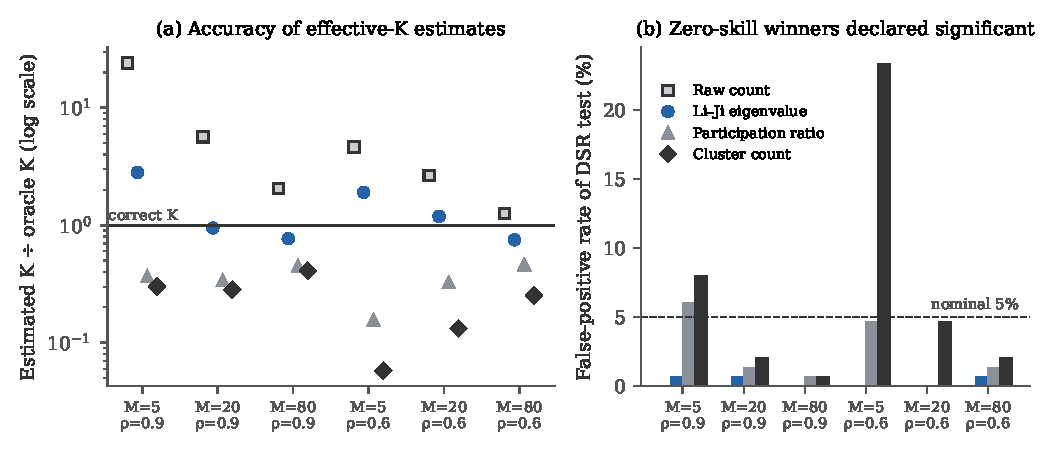
\includegraphics[width=\linewidth]{fig6.pdf}
\caption{Experiment 7. (a) Each estimator's effective $K$ relative to the oracle value (log scale; 1 = correct). The cluster count recovers the true number of clusters but understates the effective number of trials. (b) Share of zero-skill winners declared significant by the DSR using each estimate. Raw-count bars are zero.}
\label{fig:effk}
\end{figure}

\textbf{Results.} Table~\ref{tab:exp7} and Figure~\ref{fig:effk} give the central finding: \emph{the number of clusters is not the number of independent chances}. The clustering algorithm recovered the true number of clusters exactly in every replication, yet that number understated the oracle $K$ by a factor of 2.4 to 17. The reason is that each strategy's own noise, $\varepsilon_i$, gives luck additional chances inside every cluster. The understatement is largest when clusters are few and correlation within them is moderate. With five clusters at $\rho = 0.6$, the oracle $K$ is 87; using the cluster count of 5 declared 23\% of zero-skill winners significant, whereas the oracle $K$ declared none. The participation ratio also understated $K$, by a factor of 2 to 6, with false-positive rates up to 6\%.

The Li--Ji estimator stayed within a factor of 0.75 to 2.8 of the oracle and kept the false-positive rate at or below 0.7\% in every scenario. The raw count was always safe but always too conservative.

\textbf{Power.} A correction is useful only if it still finds real skill. Figure~\ref{fig:power} shows how often the one skilled strategy was both selected and declared significant, averaged over the six scenarios. Three results stand out. First, the Li--Ji estimator's power was almost identical to that of the oracle $K$: 60.6\% against 62.1\% at a Sharpe ratio of 2.0, 18.6\% against 22.1\% at 1.5, and within 2.4 percentage points of the oracle on average across all 24 cases. Because the expected maximum grows only with the logarithm of $K$, an estimate within a factor of three costs little power, whereas an error of 17 times matters. The raw count lost a substantial share, detecting 44.6\% at 2.0 and 9.3\% at 1.5. Second, the cluster count and participation ratio detected most often (80.0\% and 74.7\% at 2.0), but this is the other side of their false positives: a test that is too lenient also passes real strategies more often. Third, and most important, no estimator rescues weak signals. With 400 trials and five years of data, a strategy with a true Sharpe ratio of 1.0 was selected in only 39\% of replications and confirmed in 2.4\% on average even with the oracle $K$; at 0.5 it was effectively invisible. The binding constraint is the amount of data, not the choice of estimator, as the Minimum Backtest Length of Section~3.3 predicts.

\begin{figure}[t]
\centering
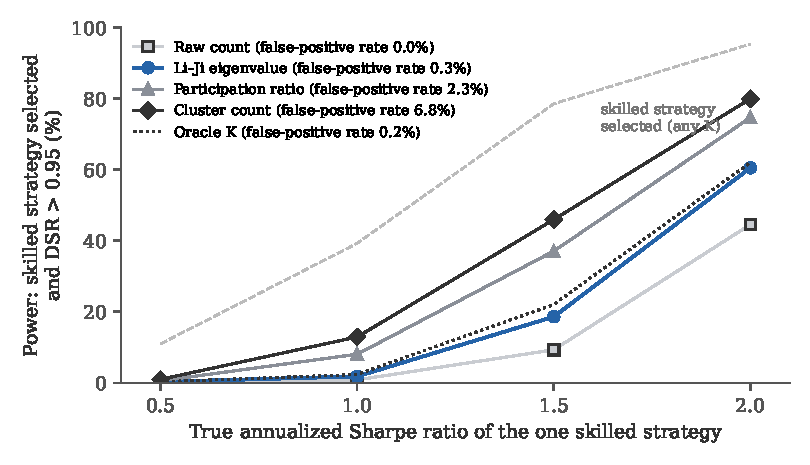
\includegraphics[width=0.85\linewidth]{fig8.pdf}
\caption{Experiment 7, power. Share of replications in which the one skilled strategy is selected and declared significant (DSR $> 0.95$), by its true Sharpe ratio, averaged over the six scenarios (120 replications each). Legend values are the mean false-positive rates from Table~\ref{tab:exp7}. The dashed grey line shows how often the skilled strategy was selected at all.}
\label{fig:power}
\end{figure}

Two further points matter for practice. First, even with the oracle $K$, the DSR's false-positive rate is close to zero rather than 5\%, because it compares the winner with the \emph{expected} maximum rather than an upper quantile of the maximum. This built-in conservatism hides moderate errors in $K$, but not an error of 17 times, and it also costs power. Second, the eigenvalue estimator comes from genetics, where correlated tests are routine; the transfer is natural because the problem, many correlated tests of one hypothesis family, is the same.



%=====================================================
\section{Real-data case study: timing the S\&P 500}\label{sec:real}

\textbf{Data and design.} The simulations have a known truth; real data do not, so this section illustrates the tools rather than proving anything. I use daily closes of the S\&P~500 price index (Yahoo Finance, ticker \textasciicircum GSPC) from January 1990 to 29 September 2026, 9{,}253 observations. The same 156 crossover rules are used as long-or-cash timing rules: long the index when the fast average is above the slow one, otherwise in cash, which earns zero. Moving-average rules of this kind have a long history in the literature \citep{brock1992,sullivan1999}. Each change of position costs 2 basis points. Rules are selected on 1990--2010 (after a 200-day warm-up) and evaluated on 2011--2026. Buy-and-hold is the natural benchmark.

\textbf{Results.} The in-sample winner was the 50/200-day crossover, the well-known ``golden cross''. Over 1990--2010 its Sharpe ratio was 0.66, against 0.38 for buy-and-hold, and 74\% of all rules beat buy-and-hold. Over 2011--2026 the winner's Sharpe ratio fell to 0.52, against 0.67 for buy-and-hold; it ranked only at the 35th percentile of the 156 rules, and just 6\% of rules beat buy-and-hold (Figure~\ref{fig:sp500}). The in-sample advantage over the benchmark disappeared.

\begin{figure}[t]
\centering
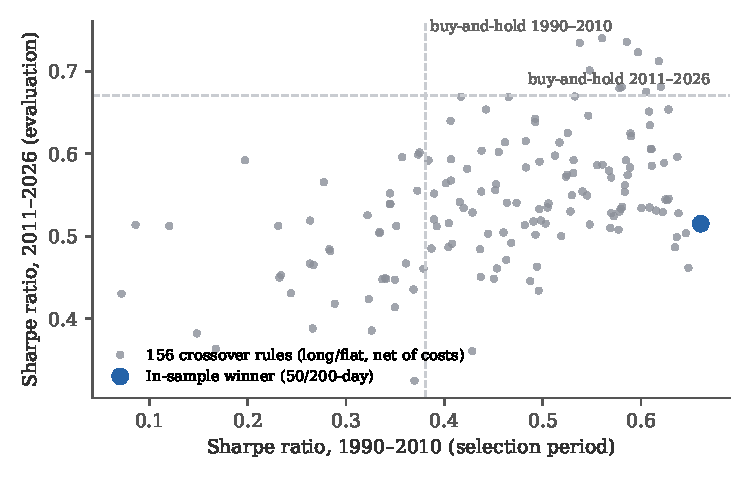
\includegraphics[width=0.8\linewidth]{fig7.pdf}
\caption{S\&P~500 case study. Sharpe ratio of each long/cash crossover rule in the selection period (horizontal axis) and evaluation period (vertical axis), net of 2 bps costs. Dashed lines mark buy-and-hold in each period. Index prices exclude dividends; cash earns zero.}
\label{fig:sp500}
\end{figure}

\begin{table}[h]
\centering
\caption{S\&P~500 case study. Deflated Sharpe Ratio of the in-sample winner (1990--2010) under different estimates of the effective number of trials. ``Cross-sectional'' uses the variance of the 156 rules' Sharpe ratios; ``null'' uses $1/T$.}
\label{tab:sp500}
\small
\begin{tabular}{lrcc}
\toprule
Estimate of $K$ & $K$ & DSR (cross-sectional variance) & DSR (null variance) \\
\midrule
Raw count & 156 & 0.92 & 0.61 \\
Li--Ji eigenvalue & 20 & 0.97 & 0.86 \\
Cluster count & 2 & 0.996 & 0.99 \\
Participation ratio & 1.5 & 0.998 & 0.997 \\
\midrule
Naive PSR (no correction) & 1 & \multicolumn{2}{c}{0.998} \\
\bottomrule
\end{tabular}
\end{table}

Table~\ref{tab:sp500} shows how much the statistical verdict depends on the choice of $K$. Because all long-or-cash rules hold the market most of the time, their returns are highly correlated, and the cluster count and participation ratio judge them to be one or two independent trials. With those estimates the winner looks highly significant. With the raw count it fails at the 5\% level. The Li--Ji estimate falls in between and passes only with the cross-sectional variance. Two further cautions apply. The DSR here tests against a Sharpe ratio of zero, whereas the economically relevant benchmark is buy-and-hold, which the winner did not beat out of sample. And the PBO of the full search was 0.40: rankings were somewhat persistent, with an in-sample/out-of-sample rank correlation of 0.47, but what persisted was mainly exposure to the market, not outperformance of it. The case illustrates Experiment~7's lesson on real data: an optimistic estimate of $K$ can turn a search result into an apparently significant discovery.

%=====================================================
\section{How ML pipelines manufacture false strategies}\label{sec:ml}

The experiments isolate a few mechanisms. In practice they occur together, and most are invisible in a final report.

\begin{enumerate}[leftmargin=*]
\item \textbf{Unrecorded trials.} Hyperparameter tuning, feature selection, early-stopping choices, alternative labels and repeated reruns with different random seeds are all trials. Experiment~5 shows that 200 such configurations are enough to produce a validation Sharpe ratio above 2 from pure noise. Automated tools (grid search, Bayesian optimisation, AutoML) can run thousands without the researcher looking at most of them. If only the final configuration is reported, the reader cannot apply any correction, because $K$ is unknown.
\item \textbf{Leakage through overlapping labels.} As Experiment 4 shows, labels defined over future windows create dependence between nearby observations. Standard $k$-fold cross-validation assumes independent observations and therefore overstates accuracy \citep{lopezdeprado2018}.
\item \textbf{Look-ahead and survivorship bias.} Features computed with information not available at the time (revised macroeconomic data, end-of-day prices used for same-day decisions, index constituents chosen with hindsight) create performance that cannot be realised.
\item \textbf{Using the test set more than once.} Each time a held-out set is consulted and the model is then revised, the hold-out becomes part of the training process. After enough iterations, ``out-of-sample'' results are in-sample results with extra steps.
\item \textbf{Non-stationarity.} Market regimes, microstructure and participants change. A pattern that was real in one period may vanish or reverse, and a long backtest may average over regimes that no longer exist. This limits the cure of simply collecting more data.
\item \textbf{Low signal-to-noise ratio.} In image recognition the signal is strong and an overfit model is quickly exposed. In return prediction, a genuine edge may explain well under 1\% of variance \citep{gu2020}, so noise dominates every estimate and the dispersion term in Eq.~\eqref{eq:fst} is large.
\item \textbf{Selective reporting and publication incentives.} Journals, funds and employers reward impressive backtests. This acts as a second, institutional layer of selection on top of the researcher's own search \citep{harvey2016,ioannidis2005}.
\end{enumerate}

%=====================================================
\section{Defences: a validation protocol}\label{sec:protocol}

No single statistic solves the problem. The following protocol combines established tools, following \citet{arnott2019}, \citet{lopezdeprado2018} and \citet{lopezdeprado2019crisis}, with the lessons of Experiments 5--7. It is split into core requirements, which every project needs and which cost little, and statistical safeguards, which quantify how much evidence remains after search.

\paragraph{Core requirements.}
\begin{enumerate}[leftmargin=*]
\item \textbf{State the hypothesis first.} Write down the economic mechanism that should produce the effect, and the test that would falsify it, before running the backtest. A strategy without a reason to exist is the most likely to be a false discovery.
\item \textbf{Register every trial.} Log every configuration evaluated, including failed ones and reruns with new seeds, with its return series. Without this log, $K$ is unknown and none of the safeguards below can be applied.
\item \textbf{Validate in time, not at random.} Use purged and embargoed cross-validation, walk-forward testing, or combinatorial purged cross-validation \citep{lopezdeprado2018}. Never shuffle dependent financial observations across folds.
\item \textbf{Hold out a final sample that is used once.} Reserve the most recent data, touch it once after all decisions are fixed, and report the result whatever it is \citep{cawley2010}. Then follow with a period of paper trading or small-scale live trading.
\item \textbf{Compare with the right benchmark and include frictions.} Judge a strategy against the simple alternative an investor could hold instead, such as buy-and-hold, and deduct transaction costs, slippage, borrowing costs and capacity limits.
\end{enumerate}

\paragraph{Statistical safeguards.}
\begin{enumerate}[leftmargin=*,resume]
\item \textbf{Estimate the effective number of trials conservatively.} Compute an eigenvalue-based estimate such as Li--Ji, Eq.~\eqref{eq:liji}, from the logged return series. Do not rely on a cluster count alone, and report how the conclusion changes between the raw count and the estimate (Experiment~7, Table~\ref{tab:sp500}).
\item \textbf{Deflate the headline statistic.} Report the Deflated Sharpe Ratio, Eq.~\eqref{eq:psr} with $SR^*$ from Eq.~\eqref{eq:fst}, rather than the raw Sharpe ratio. For factor research, use a multiple-testing threshold such as $t > 3.0$ \citep{harvey2016} or a false-discovery-rate procedure \citep{benjamini1995}.
\item \textbf{Measure the probability of overfitting.} Compute PBO with CSCV \citep{bailey2017pbo}. A PBO near 0.5 or above means the selection procedure is no better than chance.
\item \textbf{Check the backtest length.} Compare the sample length with the Minimum Backtest Length, Eq.~\eqref{eq:minbtl}, for the effective number of trials. If the data are too short, the honest conclusion is that the evidence is insufficient.
\item \textbf{Test against a family-wise benchmark.} Where many models compete, use White's Reality Check, Hansen's SPA test or the Romano--Wolf stepwise procedure \citep{white2000,hansen2005,romano2005}.
\end{enumerate}

%=====================================================
\section{Discussion and conclusion}\label{sec:disc}

\paragraph{Summary.} The experiments confirm, with known ground truth, what the theory predicts, and extend it in three directions. Searching over worthless strategies reliably produces impressive backtests, and the inflation grows with the number of trials as the False Strategy Theorem predicts. The same happens when the search is over ML models: 200 configurations of four model families produced validation Sharpe ratios above 2 on unpredictable data, and none survived an untouched test year. Realistic volatility, regime changes and transaction costs did not change these conclusions. Naive significance tests offered no protection; deflated statistics did, but only if the effective number of trials was estimated well. Counting clusters of similar strategies understated it by up to 17 times and raised the false-positive rate to 23\%, whereas an eigenvalue estimator from genetics controlled false positives and came within a few percentage points of the best achievable power. No estimator, however, could detect a genuine Sharpe ratio of 1.0 among 400 trials with five years of data. On the S\&P~500, the best of 156 timing rules beat buy-and-hold in sample and trailed it out of sample, and its deflated significance depended heavily on how the trials were counted.

\paragraph{Limitations.} Most experiments use synthetic data. This is deliberate, since only synthetic data have a known truth, but the processes are still simplifications: Experiment~6 adds volatility clustering, regimes and heavy tails, but not cross-sectional dependence across many assets, changing correlations or market impact. The ML search in Experiment~5 uses 200 configurations and small models, far fewer than an industrial AutoML run; since inflation grows with the number of trials, larger searches would be expected to inflate more. The effective-$K$ study uses one stylised correlation structure, equal clusters with one factor each, and a simplified clustering step; real strategy libraries are messier, and the oracle $K$ is defined through the theorem's approximation. The power analysis places a single skilled strategy among zero-skill ones; libraries with many weakly skilled strategies may behave differently. The real-data study uses one index, one split and price returns without dividends, so it is an illustration, not a test of technical analysis. Finally, this paper does not claim that ML has no value in finance. \citet{gu2020}, \citet{kelly2024} and \citet{jensen2023} provide evidence that carefully validated models and factors can capture real effects. The argument is narrower: the burden of proof rises with the size of the search, and a reported backtest that does not account for its search may not provide enough evidence that its performance will survive.

\paragraph{Future work.} Natural extensions include testing the effective-$K$ estimators on logged trials from real research pipelines, studying their behaviour when clusters differ in size and strength, and deriving a version of the DSR that uses an upper quantile of the maximum rather than its expectation, which would give a test with an exact error rate. A further question is how these tools apply beyond finance. Any field that combines flexible models, many analysis choices and noisy, non-repeatable data, including computational neuroscience and genomics, faces a version of the same problem, and Experiment~7 suggests that methods can usefully travel between these fields.

\paragraph{Conclusion.} In finance, discovering a strategy that worked in the past is easy; discovering one that \emph{will} work is hard, and the difference between the two grows with every additional model one tries. The response is not to abandon ML but to account honestly for search: record every trial, estimate how many independent chances luck has had, deflate every headline statistic, validate in time, and treat an impressive backtest as a hypothesis, not a result.

\paragraph{Use of AI tools.} The author used the assistance of AI (Claude, by Anthropic) while preparing this paper and its code, and takes full responsibility for the content.

%=====================================================
\begin{thebibliography}{99}\setlength{\itemsep}{0pt}\footnotesize

\bibitem[Arnott et~al.(2019)]{arnott2019}
Arnott, R., Harvey, C.~R., \& Markowitz, H. (2019). A backtesting protocol in the era of machine learning. \emph{Journal of Financial Data Science}, 1(1), 64--74.

\bibitem[Bailey and L\'opez de Prado(2012)]{bailey2012}
Bailey, D.~H., \& L\'opez de Prado, M. (2012). The Sharpe ratio efficient frontier. \emph{Journal of Risk}, 15(2), 3--44.

\bibitem[Bailey and L\'opez de Prado(2014)]{bailey2014dsr}
Bailey, D.~H., \& L\'opez de Prado, M. (2014). The deflated Sharpe ratio: Correcting for selection bias, backtest overfitting, and non-normality. \emph{Journal of Portfolio Management}, 40(5), 94--107.

\bibitem[Bailey et~al.(2014)]{bailey2014pseudo}
Bailey, D.~H., Borwein, J.~M., L\'opez de Prado, M., \& Zhu, Q.~J. (2014). Pseudo-mathematics and financial charlatanism: The effects of backtest overfitting on out-of-sample performance. \emph{Notices of the American Mathematical Society}, 61(5), 458--471.

\bibitem[Bailey et~al.(2017)]{bailey2017pbo}
Bailey, D.~H., Borwein, J.~M., L\'opez de Prado, M., \& Zhu, Q.~J. (2017). The probability of backtest overfitting. \emph{Journal of Computational Finance}, 20(4), 39--69.

\bibitem[Benjamini and Hochberg(1995)]{benjamini1995}
Benjamini, Y., \& Hochberg, Y. (1995). Controlling the false discovery rate: A practical and powerful approach to multiple testing. \emph{Journal of the Royal Statistical Society: Series B}, 57(1), 289--300.

\bibitem[Bergstra and Bengio(2012)]{bergstra2012}
Bergstra, J., \& Bengio, Y. (2012). Random search for hyper-parameter optimization. \emph{Journal of Machine Learning Research}, 13, 281--305.

\bibitem[Bollerslev(1986)]{bollerslev1986}
Bollerslev, T. (1986). Generalized autoregressive conditional heteroskedasticity. \emph{Journal of Econometrics}, 31(3), 307--327.

\bibitem[Brock et~al.(1992)]{brock1992}
Brock, W., Lakonishok, J., \& LeBaron, B. (1992). Simple technical trading rules and the stochastic properties of stock returns. \emph{Journal of Finance}, 47(5), 1731--1764.

\bibitem[Cawley and Talbot(2010)]{cawley2010}
Cawley, G.~C., \& Talbot, N.~L.~C. (2010). On over-fitting in model selection and subsequent selection bias in performance evaluation. \emph{Journal of Machine Learning Research}, 11, 2079--2107.

\bibitem[Gu et~al.(2020)]{gu2020}
Gu, S., Kelly, B., \& Xiu, D. (2020). Empirical asset pricing via machine learning. \emph{Review of Financial Studies}, 33(5), 2223--2273.

\bibitem[Hamilton(1989)]{hamilton1989}
Hamilton, J.~D. (1989). A new approach to the economic analysis of nonstationary time series and the business cycle. \emph{Econometrica}, 57(2), 357--384.

\bibitem[Hansen(2005)]{hansen2005}
Hansen, P.~R. (2005). A test for superior predictive ability. \emph{Journal of Business \& Economic Statistics}, 23(4), 365--380.

\bibitem[Harvey et~al.(2016)]{harvey2016}
Harvey, C.~R., Liu, Y., \& Zhu, H. (2016). \ldots and the cross-section of expected returns. \emph{Review of Financial Studies}, 29(1), 5--68.

\bibitem[Holm(1979)]{holm1979}
Holm, S. (1979). A simple sequentially rejective multiple test procedure. \emph{Scandinavian Journal of Statistics}, 6(2), 65--70.

\bibitem[Hou et~al.(2020)]{hou2020}
Hou, K., Xue, C., \& Zhang, L. (2020). Replicating anomalies. \emph{Review of Financial Studies}, 33(5), 2019--2133.

\bibitem[Ioannidis(2005)]{ioannidis2005}
Ioannidis, J.~P.~A. (2005). Why most published research findings are false. \emph{PLoS Medicine}, 2(8), e124.

\bibitem[Jensen et~al.(2023)]{jensen2023}
Jensen, T.~I., Kelly, B., \& Pedersen, L.~H. (2023). Is there a replication crisis in finance? \emph{Journal of Finance}, 78(5), 2465--2518.

\bibitem[Kelly et~al.(2024)]{kelly2024}
Kelly, B., Malamud, S., \& Zhou, K. (2024). The virtue of complexity in return prediction. \emph{Journal of Finance}, 79(1), 459--503.

\bibitem[Li and Ji(2005)]{liji2005}
Li, J., \& Ji, L. (2005). Adjusting multiple testing in multilocus analyses using the eigenvalues of a correlation matrix. \emph{Heredity}, 95(3), 221--227.

\bibitem[Lo(2002)]{lo2002}
Lo, A.~W. (2002). The statistics of Sharpe ratios. \emph{Financial Analysts Journal}, 58(4), 36--52.

\bibitem[Lo and MacKinlay(1990)]{lo1990}
Lo, A.~W., \& MacKinlay, A.~C. (1990). Data-snooping biases in tests of financial asset pricing models. \emph{Review of Financial Studies}, 3(3), 431--467.

\bibitem[L\'opez de Prado(2018)]{lopezdeprado2018}
L\'opez de Prado, M. (2018). \emph{Advances in Financial Machine Learning}. Hoboken, NJ: Wiley.

\bibitem[L\'opez de Prado(2019)]{lopezdeprado2019crisis}
L\'opez de Prado, M. (2019). A data science solution to the multiple-testing crisis in financial research. \emph{Journal of Financial Data Science}, 1(1), 99--110.

\bibitem[L\'opez de Prado and Bailey(2021)]{lopezdeprado2021fst}
L\'opez de Prado, M., \& Bailey, D.~H. (2021). The false strategy theorem: A financial application of experimental mathematics. \emph{American Mathematical Monthly}, 128(9), 825--831.

\bibitem[L\'opez de Prado and Lewis(2019)]{lopezdeprado2019lewis}
L\'opez de Prado, M., \& Lewis, M.~J. (2019). Detection of false investment strategies using unsupervised learning methods. \emph{Quantitative Finance}, 19(9), 1555--1565.

\bibitem[McLean and Pontiff(2016)]{mclean2016}
McLean, R.~D., \& Pontiff, J. (2016). Does academic research destroy stock return predictability? \emph{Journal of Finance}, 71(1), 5--32.

\bibitem[Romano and Wolf(2005)]{romano2005}
Romano, J.~P., \& Wolf, M. (2005). Stepwise multiple testing as formalized data snooping. \emph{Econometrica}, 73(4), 1237--1282.

\bibitem[Sullivan et~al.(1999)]{sullivan1999}
Sullivan, R., Timmermann, A., \& White, H. (1999). Data-snooping, technical trading rule performance, and the bootstrap. \emph{Journal of Finance}, 54(5), 1647--1691.

\bibitem[White(2000)]{white2000}
White, H. (2000). A reality check for data snooping. \emph{Econometrica}, 68(5), 1097--1126.

\end{thebibliography}
\end{document}
